\section{引言}

多视图几何重建旨在从无序或有序的多张图像中恢复场景的三维结构、相机内外参数以及与场景几何相关的中间表示，是从二维视觉观测走向三维世界理解的基础问题。对这一方向而言，核心任务并不只是“估计深度”或“回归位姿”，而是要在缺乏直接深度传感的前提下，利用跨视角投影关系，把分散的二维像素组织成一个几何上自洽、全局上一致、并可被下游任务复用的三维场景解释。传统方法通常遵循“特征提取与匹配、相机注册、三角化与光束法平差”的经典管线，其中 Bundle Adjustment 被视为保证全局一致性的关键环节\cite{triggs2000bundle,schoenberger2016colmap}。然而，这一管线高度依赖手工设计的特征与多阶段优化，面对弱纹理、遮挡、宽基线与大规模图像集合时，往往在鲁棒性、效率与泛化性上面临明显瓶颈\cite{wang2021deep2view,wang2024vggsfm}。

近五年，多视图几何重建逐步出现“学习化”趋势：研究者不再仅将深度网络作为传统流程的局部替代模块，而是尝试让网络直接参与几何对应、相机估计、全局优化乃至统一几何属性预测\cite{bhalgat2023lighttouch,karaev2024cotracker,wang2025vggt}。在这一演进过程中，学习方法的价值不只是“把某个模块做得更准”，而是重新回答三个相互关联的问题：如何获得更稳定的跨视角对应，如何让全局求解既保持几何约束又具备可学习性，以及如何把原本割裂的几何变量组织为可迁移的统一表示\cite{wang2024vggsfm,wang2025vggt}。也正因如此，多视图几何重建正在从传统的工程化流水线问题，逐渐转变为“几何结构如何被学习模型吸收和重组”的方法论问题。

在众多研究团队中，Oxford Visual Geometry Group（VGG）围绕这一主题形成了较为清晰且连续的研究主线。其工作并非对传统几何的简单替代，而是强调将多视图几何的结构性约束、对应关系与优化逻辑逐步转移到学习框架内部。从早期强调几何先验与任务设定的工作\cite{wu2020unsup3d,wang2021deep2view}，到关注点轨迹与跨视角关系建模的 CoTracker 系列\cite{karaev2024cotracker,karaev2025cotracker3}，再到将结构恢复系统整体可微化的 VGGSfM\cite{wang2024vggsfm}以及面向统一几何属性预测的 VGGT\cite{wang2025vggt}，VGG 团队的成果较完整地呈现了多视图几何重建“学习化”的方法演进。与只在单点任务上取得突破的工作相比，这条主线更适合被当作一个可分析的样本，因为它不仅包含代表性论文，更包含论文之间清晰的前后承接关系。

基于课程要求，本文选择“多视图几何重建中的学习方法”作为明确研究主题，以 VGG 团队为代表案例展开综述，而不是泛泛介绍整个团队的三维视觉工作。全文将重点回答以下问题：多视图几何重建这一方向为什么值得持续研究；它主要试图解决哪些核心问题；学习方法究竟改造了传统管线中的哪些关键环节；以及 VGG 团队的代表性成果如何形成一条层层递进的研究主线。通过这些问题，本文希望帮助读者同时理解“这个方向为什么重要”与“为什么 VGG 团队值得被单独综述”。

\subsection{研究背景与意义}

多视图几何重建广泛应用于自动驾驶、AR/VR、机器人导航、文化遗产数字化与三维内容生成等场景。相较依赖激光雷达或深度相机的主动感知方案，仅依赖普通 RGB 图像的方案具有设备廉价、部署灵活、成像分辨率高等优点，因此长期以来都是计算机视觉的重要研究方向\cite{schoenberger2016colmap,reizenstein2021co3d}。然而，图像到三维的恢复本质上是病态问题，必须借助跨视角几何约束、匹配一致性与全局优化，才能得到可信的相机与结构估计。

从应用层面看，多视图几何重建并不只是一个传统视觉任务，而是连接二维感知与三维世界理解的基础桥梁。在自动驾驶与机器人系统中，场景几何决定了障碍物定位、路径规划和交互安全；在 AR/VR 中，几何重建又直接关系到虚实对齐、遮挡关系与真实感渲染；在数字文化遗产保护与工业检测场景中，稳定而高精度的三维恢复则决定了后续建模、存档与测量分析的质量。因此，如何让仅依赖图像的三维重建方法变得更稳健、更高效、更易泛化，具有明确的工程价值与学术价值。

同时，该方向之所以长期具有研究吸引力，还在于它天然处于“物理规律”与“数据驱动学习”之间的交汇点。一方面，多视图几何由投影模型、相对运动和重投影误差等明确数学结构决定；另一方面，真实世界中的纹理缺失、反射、遮挡与动态变化，又使得纯解析方法难以覆盖全部复杂情形。也正是在这一张力下，学习方法才逐渐成为推动该方向继续发展的关键力量。

从当前技术发展背景看，这一方向之所以尤其值得在今天重新审视，还因为其正在与机器人感知、具身智能和三维内容生成等新需求发生更紧密的耦合。无论是需要实时空间理解的机器人系统，还是需要可编辑三维场景表示的生成式应用，都要求视觉系统不仅“看见”图像内容，更要获得可度量、可推理、可复用的场景几何结构。由此可见，多视图几何重建不只是一个传统问题的延续，而是在新的应用牵引下不断获得新意义的基础能力。

\subsection{核心关注点与研究难点}

该方向当前的核心难点主要包括：跨视角对应的不稳定性、增量式管线的误差累积、复杂场景下的泛化能力不足，以及大规模场景下优化成本过高等\cite{wang2021deep2view,karaev2024cotracker,wang2024vggsfm}。因此，如何在保持几何一致性的同时提高学习模型的表达能力与推理效率，构成了近年多视图几何重建研究的关键问题。

进一步细分，这些难点实际上对应多视图几何管线中的三个关键环节。第一是观测层，即如何从图像中获得高质量、可长期保持一致的对应关系；第二是求解层，即如何在相机恢复、三角化与全局优化阶段维持数值稳定与几何可解释性；第三是表示层，即如何让模型输出的几何结果既便于重建本身，也能够服务于深度估计、跟踪、视图合成和动态场景理解等下游任务。VGG 团队近五年的工作，恰恰可以被理解为分别围绕这三个环节逐步展开。

此外，近两年该方向又新增了一类重要问题，即统一性问题。过去多视图几何系统更倾向于“一个模块做一件事”，而当前越来越多方法开始尝试让同一模型同时处理相机参数、深度、点图和轨迹等多种属性\cite{wang2025vggt,wang2024dust3r,mast3r2024}。这意味着研究目标已经从“单模块精度提升”逐步转向“统一场景几何表示的构建”，这也是本文在综述中将 VGGSfM 和 VGGT 视为关键节点的重要原因。

若从更本质的层面概括，这一方向所面对的其实是三组长期存在的矛盾。其一是“局部观测有限”与“全局几何一致”之间的矛盾，即单个像素或局部匹配信息往往十分脆弱，但最终恢复出的相机和结构却必须满足全局自洽。其二是“显式优化可靠”与“计算代价高昂”之间的矛盾，即传统几何求解具有可解释性，却往往难以满足大规模和高效率需求。其三是“统一表示更具复用性”与“训练监督更复杂”之间的矛盾，即模型越希望一次性输出更多几何属性，就越需要更强的数据、监督和模型设计来维持一致性。当前多视图几何重建研究的核心关注点，正是在这三组矛盾之间寻找新的平衡。

\subsection{选择 VGG 团队作为综述对象的原因}

VGG 团队在该方向的工作具有三个适合作为综述案例的特征。第一，其研究主题高度集中，长期围绕几何先验、跨视角对应、SfM 系统学习化与统一几何表示展开。第二，其代表论文之间存在明显的递进关系，适合从“问题链条”而非“论文堆砌”角度组织综述。第三，其工作发表在 CVPR、ICCV、ECCV 等高水平会议，并普遍提供论文、项目页或代码，便于基于一级来源进行核实与写作\cite{bhalgat2023lighttouch,wang2024vggsfm,wang2025vggt}。

更重要的是，VGG 团队的方法路径具有较强的代表性和可分析性。与某些仅在单一任务或单一模型上取得突破的研究不同，VGG 团队的工作覆盖了数据、表征、几何求解与统一预测等多个层面，因而能够较完整地反映当前多视图几何重建学习化的总体趋势。与此同时，这条研究主线又保持了足够清晰的边界，使本文可以围绕“多视图几何重建中的学习方法”这一明确主题展开，而不会滑向泛泛的“某团队视觉研究综述”。

进一步说，选择 VGG 团队并不是因为它“覆盖面最广”，而是因为它恰好沿着本文最关心的研究链条持续推进。许多优秀团队也在多视图重建、NeRF、三维生成或视觉基础模型上取得了重要成果，但未必同时呈现出从几何先验、对应学习、系统求解到统一表示这一完整而连续的演进关系。相比之下，VGG 团队的价值在于：其代表性成果之间不仅共享主题，更共享一个可被清晰复原的问题推进逻辑，即前一阶段暴露出的瓶颈，往往直接构成后一阶段工作的出发点。

这使 VGG 团队特别适合作为课程综述对象。对于一篇强调“把研究内容讲清楚、把论文关系讲清楚、把发展逻辑讲清楚”的课程报告而言，最理想的样本不是论文数量最多的团队，而是能够帮助读者看见研究主线如何展开的团队。VGG 的研究路径恰好具备这种教学意义：它既足够前沿，能够反映近五年多视图几何重建的关键转向；又足够连贯，能够支撑从“为什么值得研究”一路分析到“未来可能如何发展”。

\begin{figure}[H]
  \centering
  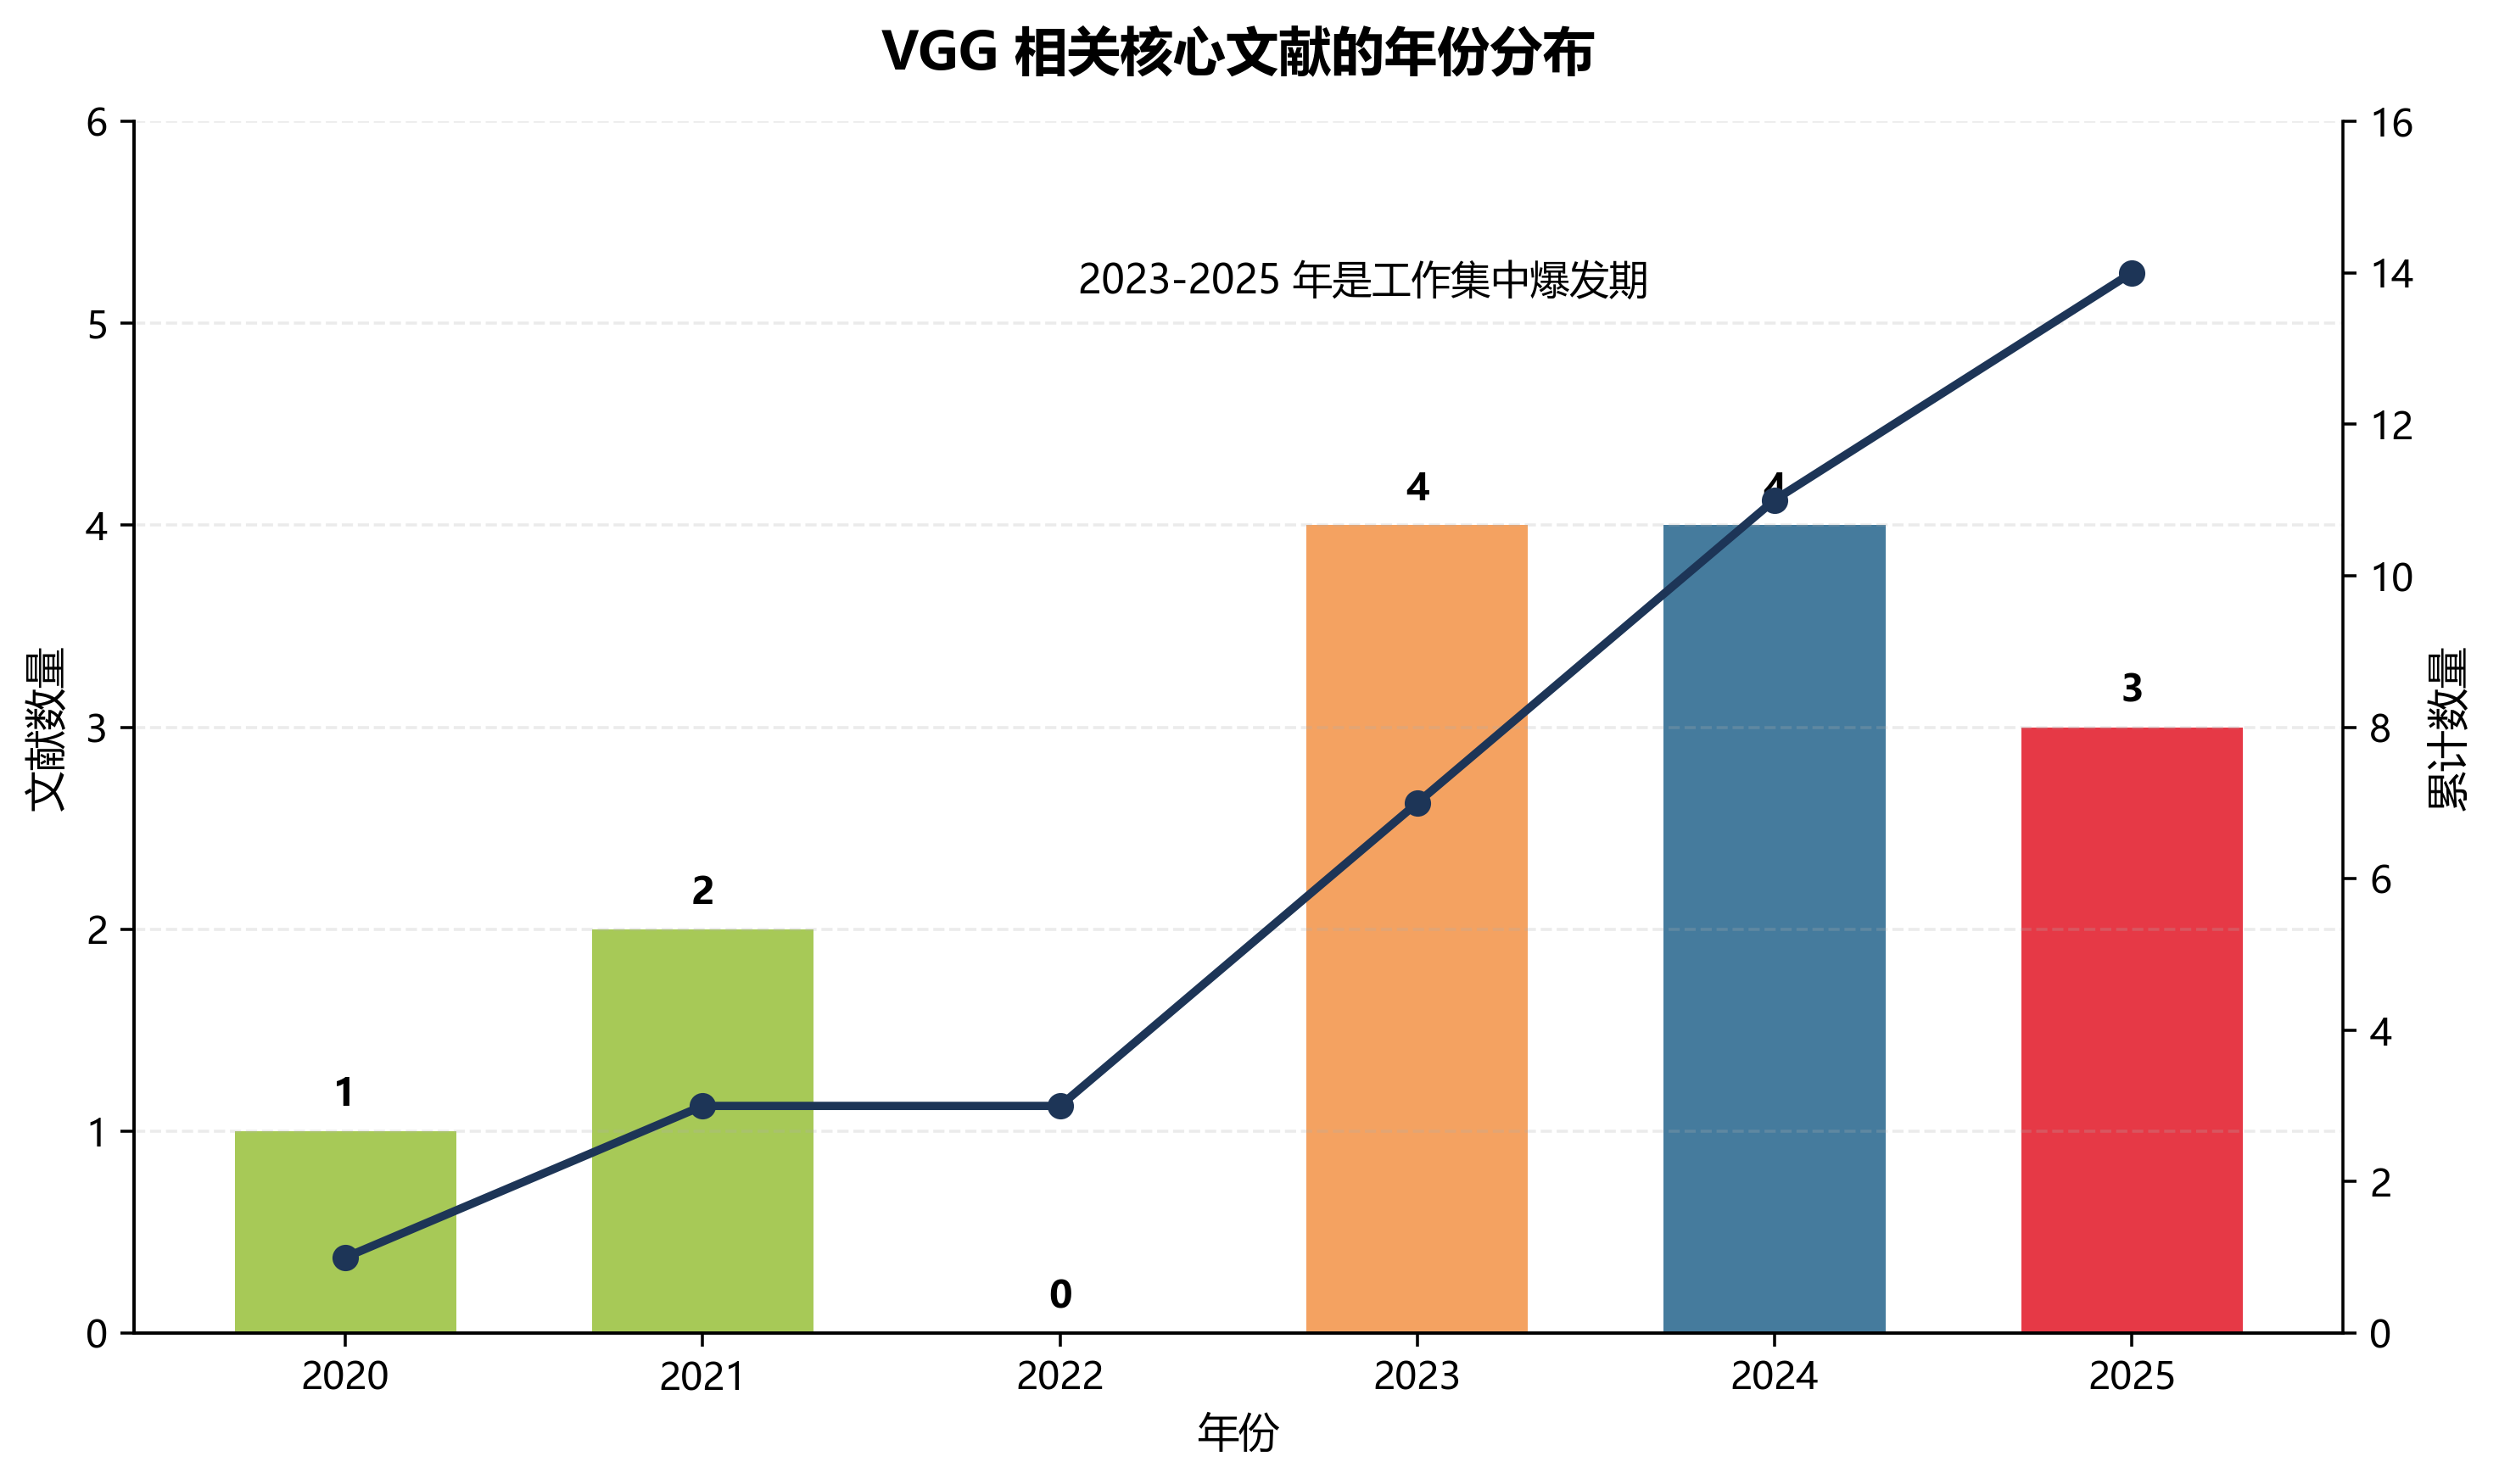
\includegraphics[width=10.8cm]{figures/vgg_year_distribution.png}
  \BiCaption{VGG 相关核心文献的年份分布}{Year-wise Distribution of Core VGG-related References}
  \label{fig:vgg-year-distribution}
\end{figure}

从文献时间分布上看，如图~\ref{fig:vgg-year-distribution} 所示，VGG 团队与本文主题直接相关的核心工作主要集中在 2023--2025 年。这一现象说明该研究方向并非长期稳定的传统子领域，而是在近几年随着 Transformer、点轨迹学习和统一几何预测方法的发展而快速升温。换言之，本文所综述的并不是一个已经完全定型的成熟方向，而是一条仍在快速延展、且研究范式仍在变化中的新兴主线。

如果进一步观察图中堆叠柱的内部构成，还可以发现数量增长并不是平均发生的，而是伴随着研究重心的阶段性迁移。2020--2021 年的代表工作主要集中在几何先验、任务设定与数据基础层面，说明该阶段的重点是回答“什么问题值得学、用什么数据来学、哪些几何结构不能丢”；2023--2024 年的新增工作则明显集中在对应关系和点轨迹建模上，说明团队开始优先修补传统管线中最脆弱的观测环节；直到 2024--2025 年，系统重构与统一输出相关工作才真正集中出现。这意味着 VGG 主线的推进并不是围绕单一模型持续做局部改良，而是沿着“观测—求解—表示”的问题链条不断上移。

\begin{figure}[H]
  \centering
  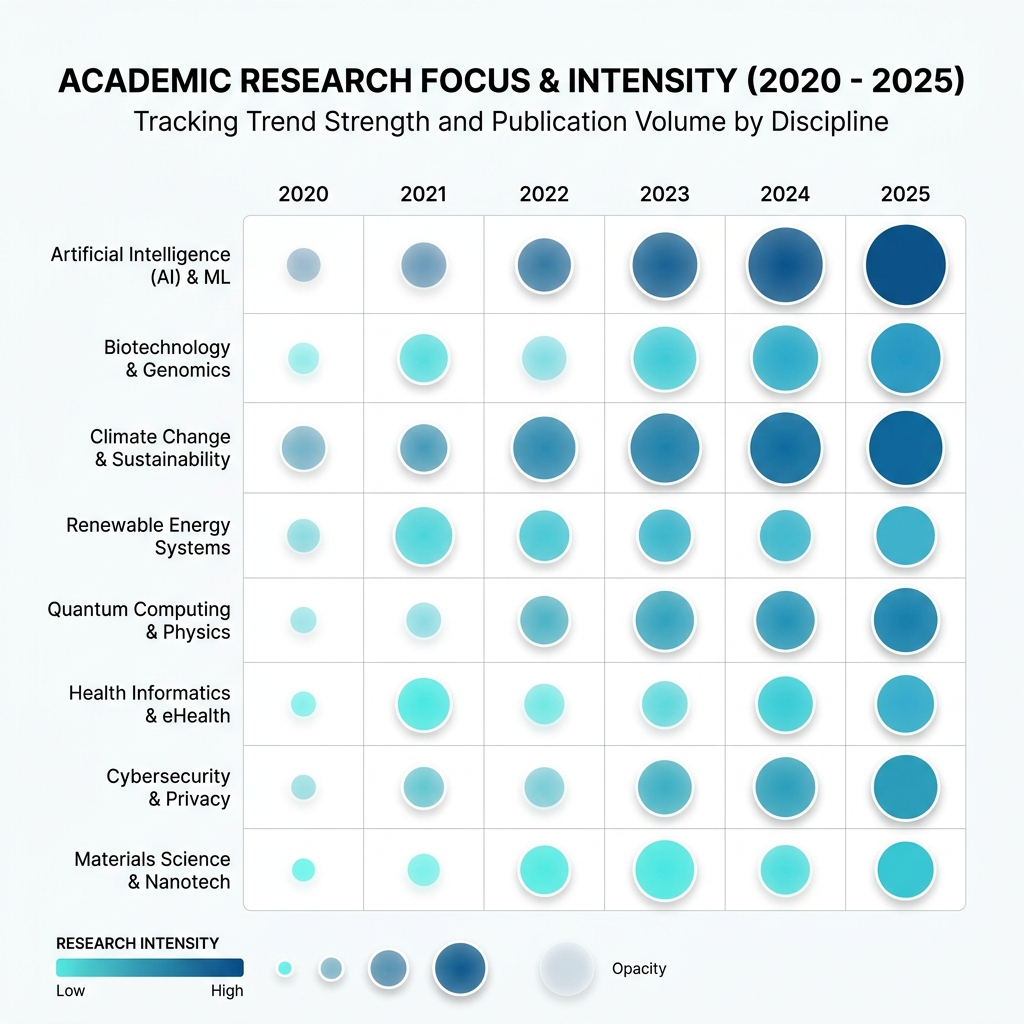
\includegraphics[width=11.2cm]{figures/vgg_focus_heatmap.png}
  \BiCaption{VGG 相关文献的研究重心分布热图}{Heatmap of Research Focus in Core VGG-related References}
  \label{fig:vgg-focus-heatmap}
\end{figure}

图~\ref{fig:vgg-focus-heatmap} 进一步把这种迁移关系表达得更清楚。若只看年份，读者可能会把这一主线理解为“近两年论文变多了”；但若结合研究重心类别，就会发现真正重要的变化在于论文所处理的问题层级发生了变化：早期更重视归纳偏置和数据基座，中期重视轨迹化观测与系统求解，后期则开始把统一几何表示和动态扩展纳入同一框架。按照课程报告对“研究思路如何逐步推进”的要求，这一点尤其关键，因为它解释了为什么本文不能简单按年份罗列文献，而必须按方法作用于管线的层次来组织。
